% reducesymm/elton/Arxiv_paper/Lagrangian.tex   pdflatex ECHG24; biber ECHG24

\section{Lagrangian dynamics}
\label{s:Lagrangian}

We know of the existence of  \stagp s in the flow of an Eulerian equilibrium 
velocity field predicted from the symmetries of \pCf. Thus the starting 
point for our investigation is clear; treating an Eulerian equilibrium velocity 
field as an autonomous dynamical system we have already identified the 
"fixed points" of the system, which we refer to in this context as the 
\stagp s.  Using the sum formula for computing velocities at any point in 
the \pCf\ domain \refeq{eqn:spectralsum}, by differentiating this formula 
it is a simple matter to compute the $[3\!\times\! 3]$ velocity gradients 
or Jacobian matrix at any point. Eigenvalues and eigenvectors of this 
matrix will provide linear stability analysis results for the {\stagp}s, 
and allow us to compute and visualize the local stable and unstable 
manifolds by starting a collection of tracer points along the directions 
of the eigenvectors, integrating them forwards and backwards in time 
(when the local tangent space is $2D$, trajectories are started 
throughout a small radius in the plane spanned by the eigenvectors). 
Though this method may underrepresent a part of the manifold for the $2D$ 
case \citep{SahVla09}, we find that the approximation works for revealing 
the interesting and relevant dynamical behaviors we seek. 

In order to investigate additional locations in the domain for which no 
movement occurs, we may numerically compute $|\bu|^{2}$ along a fine grid 
and try to ascertain regions where the velocity value falls below a given 
threshold. Then, using interpolation within these regions, any additional  
\stagp s can be pinned down. 

With the determination of the {\stagp}s and their invariant manifolds, we 
find a natural way to view the physical space of the fluid, partitioned 
into regions wherein the dynamics is dominated by the trajectories 
following closely the invariant manifolds. This provides us with a 
framework for studying how transport may occur within and between the 
different regions. 

\subsection{The upper branch Eulerian equilibrium}
\label{s:eq2}

Our analysis is carried out for the upper branch \eqv\ velocity field, 
{\tEQtwo}, at $\Reynolds = 400$. 
The cell size parameters are 
\beq   
[L_x,2,L_z]
         = \; [2\pi/1.14,2,4\pi/5]
         ~ [5.512,2,2.513].
\ee{cellW03}

To begin, we look at the evolution of Lagrangian tracers starting on a 
grid of points, shown in \reffig{fig:UBs}. The grid is chosen to lie 
in the $[y,z]$ plane, centered at $x = L_x/2$. The initial points are 
equally spaced, and offset by one position from the edge of the box. If 
the number of points is chosen to be one less than a multiple of 4, there 
will be points starting at $\xSP{1}=(L_x/2,0,L_z/4)$ and 
$\xSP{2}=(L_x/2,0,3L_z/4)$. The trajectories are integrated 
and run for a relatively short time. Just from evolving the 
grid of points alone, we begin to get a feel for the dynamics and start 
to see the formation of interesting patterns and vortical structures. 

{\tEQtwo} invariance under the symmetry group $S$, explained  in 
\refsect{s:symm_stag}, implies the existence of 4 \stagp s 
\tSP{1}--\tSP{4}, \refeq{s3lagrange}. In \reffig{fig:UBs_b} the view 
from \reffig{fig:UBs_a} has been rotated in order to reveal two of 
these \stagp s. The visualization of the behavior of trajectories near 
these fixed points reveals their  qualitative nature. The point at 
$3L_z/4$ in \reffig{fig:UBs_b} appears to be an unstable spiral, 
whereas the point at $L_z/4$ is hyperbolic. In order to verify these 
hypotheses, eigenvalues and stable/unstable manifolds for these \stagp s 
are computed. 

\begin{figure}
\centering
    \begin{subfigure}{0.98\textwidth}
    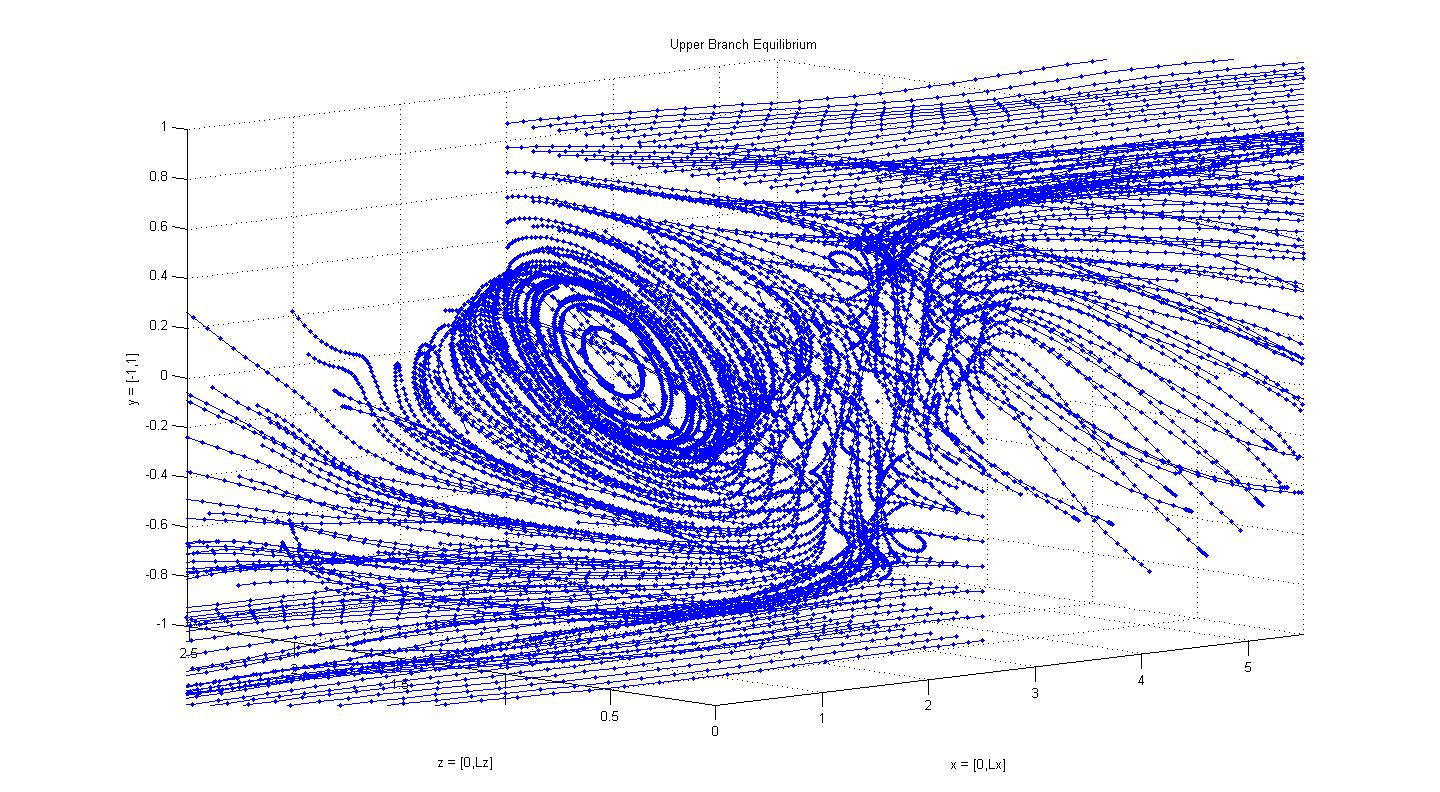
\includegraphics[width=1.0\textwidth]{fig_UB1.jpg}
      \caption{
        $3D$ perspective view
       }
      \label{fig:UBs_a}
    \end{subfigure}

    \begin{subfigure}{0.98\textwidth}
    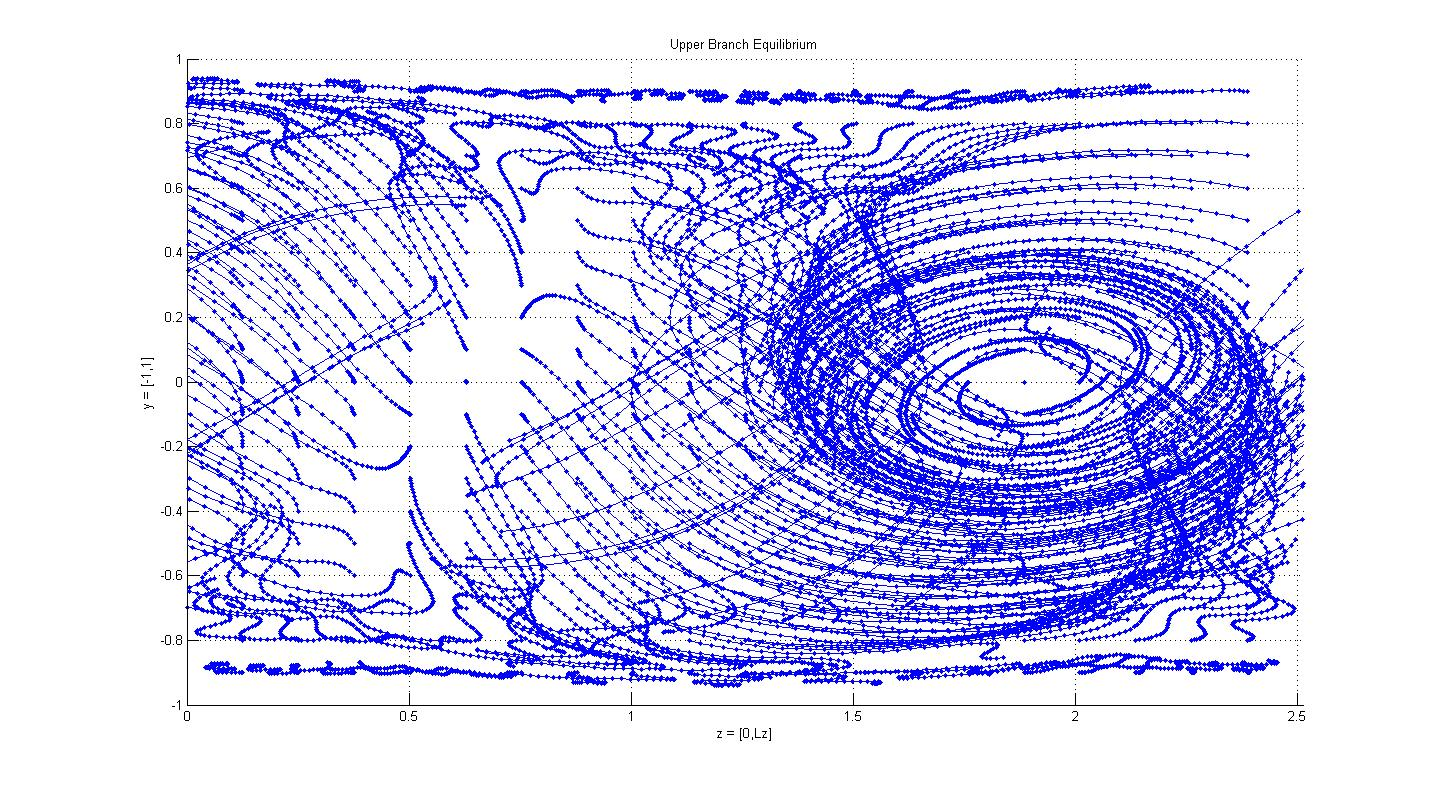
\includegraphics[width=1.0\textwidth]{fig_UB1eq.jpg}
      \caption{
        Rotated to show the 2 \stagp s
       }
      \label{fig:UBs_b}
    \end{subfigure}
    \caption{
Grid of $19 \times 19$  initial points in the $[y,z]$ plane, centered at 
$x = L_x/2$; integrated for 15 time units to produce tracer particle 
trajectories for {\tEQtwo}.} 
\label{fig:UBs}
 \end{figure}


\subsection{Linearization and stability}


For a perturbation $\delta$\bx\ away from one of the {\stagp}s,
the change in the velocity field is given by $\delta\bu = \Mvar
\delta\bx$ where $\Mvar$ is the nine component \velgradmat\ defined
by $\Mvar_{ij}=\frac{\partial u_{i}}{\partial x_{j}}$. Since \bu\ is
given by \refeq{eqn:spectralsum}, it is a relatively simple
extension of this formula to evaluate these partials. To find
$\partial\bu/\partial y$, one needs to use the relation
$\frac{\partial}{\partial y}T_{n}(y) = n U_{n-1}(y)$ where $T_{n}$
is the $n$th Chebyshev polynomial of the first kind and $U_{n}$ is
the $n$th Chebyshev polynomial of the second kind. Everything else
is straightforward.
The eigenvalues of $\Mvar$, evaluated at a {\stagp}, determine local stability
and reveal the qualitative nature of the motion nearby the \stagp.
For the \stagp s \tSP{1}--\tSP{4}, the eigenvalues, eigenvectors,
and velocity gradients matrices are as follows.

$\xSP{1}=(L_x/2,0,L_z/4)$: There are 3 real eigenvalues, two 
positive and one negative. 
\bea
\eigExp[1] &=& -0.4652099 \,,\quad
\jEigvec[1] =
\left[\begin{array}{c}
             {0.9844417} \cr
             {0.1743315} \cr
             {0.0219779}
\end{array}\right]
                                                \label{sp1_evec1} \\ 
\eigExp[2]  &=& 0.4008961 \,,\quad 
\jEigvec[2] =
\left[\begin{array}{c}
             {~~0.5704000} \cr
             {-0.7666749} \cr
             {~~0.2947091} \cr
\end{array}\right] 
                                                \label{sp1_evec2} \\  
\eigExp[3]  &=& 0.0643139 \,,\quad 
\jEigvec[3] =
\left[\begin{array}{c}
             {0.4082166} \cr
             {0.7525949} \cr
             {0.5166819} \cr
\end{array}\right]
                                                \label{sp1_evec3} 
\eea
   The \velgradmat\ is
\beq
   \Mvar =
\left[\begin{array}{ccc}
   {-0.4305385} &  {-0.3002042} &{0.8282447} \cr
   {-0.1221356} &   {0.2456107} & {-0.1675796} \cr
   {0.0001651}  &   {-0.0828951}  & {0.1849278} \cr
\end{array}\right]
\eeq
The point is a saddle; it has 1 stable dimension and a $2D$ plane of 
instability spanned by $\jEigvec[2]$ and $\jEigvec[3]$, with the 
eigenvalues summing to 0, as required by a volume-preserving flow. 
    
The \stagp\ \tSP{4} at $(0,0,3L_z/4)$ has the same eigenvalues as 
\tSP{1}. It's eigenvectors and \velgradmat\ differ by a minus sign in the 
third component (except for $\Mvar_{33}$ where the two minuses cancel). 

$\xSP{2}=(L_x/2,0,3L_z/4)$: 
There is one real, negative eigenvalue and a complex
pair with positive real part.

\bea
&\eigExp[1] = -0.0352362 \,,\quad \jEigvec[1] =
\left[\begin{array}{c}
             {-0.9452459} \cr
             {-0.1893368} \cr
             {-0.2658228} \cr
\end{array}\right]
   \\
&\eigRe[2] \pm i\,\eigIm[2] = 0.0176181 \pm i\,0.0862176
   \\
&\jEigvec[2] =
\left[\begin{array}{c}
             {0.3737950 + 0.0544113i} \cr
             {0.2098940 - 0.4925773i} \cr
             {0.7554000} \cr
\end{array}\right]
\,,\quad
\jEigvec[3] =
\left[\begin{array}{c}
             {0.3737950 - 0.0544113i} \cr
             {0.2098940 + 0.4925773i} \cr
             {0.7554000} \cr
\end{array}\right]
\nnu\,.
\eea
The \velgradmat\ is 
\[ %beq
   \Mvar =
\left[\begin{array}{ccc}
   {-0.0316935} & {-0.0708737} &  {0.0378835} \cr
  {-0.0250579} & {-0.0218884} &  {0.0795969} \cr
   {0.0014742} & {-0.1320575} &  {0.0535818} \cr
\end{array}\right]
\] %\eeq
Trajectories starting near this \stagp\ spiral out in a plane spanned by 
the complex pair of eigenvectors. The stable direction is one-dimensional 
and points primarily along the $x$ direction. 
    
\tSP{3} at $(0,0,L_z/4)$ has the same eigenvalues as \tSP{2} and again, the 
\velgradmat\ is the same except for sign changes in the third component. 
This follows from the {\pC} symmetries. 

\subsection{Further {\stagp}s}

Having analyzed {\stagp}s \tSP{1}--\tSP{4}, before further investigating the 
dynamics, one might wonder whether other such {\stagp}s may exist 
that do not necessarily follow from a symmetry argument. To answer this 
question, as mentioned above, we numerically compute $|\bu|^{2}$ along a 
fine grid and look for where its value falls below a given threshold. 

We create a more refined grid of velocities which is $144 \times 105 
\times 144$. This is three times the 48 $\times$ 35 $\times$ 48 grid in 
each dimension used to show the initial tracer trajectories, and contains 
about 2.2 million points. At each point $|\bu|^{2}$ is then calculated 
and at every point that satisfies $|\bu|^{2} < \epsilon$ for some 
arbitrarily chosen $\epsilon$, the point is plotted. 

In \reffig{fig:fine_usquare} we show regions in the cell where 
$|\bu|^{2}$ is very small for $\epsilon = 10^{-4}$, notated by the globs 
of blue dots. The trajectories shown along with the points of small 
velocity in this figure, explained below, are also suggestive of the 
existence of a {\stagp} within the spiraling region. The four previously 
known {\stagp}s are identified in the figure, but we also see a couple of 
additional clumps. Honing in one of the suspicious clusters, starting 
from the gridpoint value with smallest velocity in the suspicious region, 
$\bx_{0} \approx (2.33476, 0.40952, 0.64577)$, and its reflection through 
$\xSP{1}$, $\bx_{0}' =2 \xSP{1} - \bx_{0}$, the 
Newton iteration 
\[ %beq
 \bx_{k+1} = \bx_{k} -
          {\Mvar}^{-1}(\bx_{k}) \, \bu(\bx_{k})
\] %eeq
%  where $\Mvar$ is the \velgradmat.
converges rapidly to verify \emph{another} pair of \stagp s. Because we 
have already used notation to define points \tSP{1}--\tSP{8} in 
\refsect{s:symm_stag}, we refer to these new numerically discovered 
{\stagp}s as \tSP{N1} and \tSP{N2}: 

\bea
\xSP{N1} &=& (2.35105561774981,0.42293662349708,0.65200166068573)
\continue
\xSP{N2} &=& (3.16051044117966,-0.42293662349708,0.60463540075018)
\label{eqn:newspNewt}
\,.
\eea
%         = [5.51156605892946182182,2,2.51327412287183459075]
We see the
 symmetry in the $y$-component of this pair, and in fact
these points are shown to be
 symmetric about the point \tSP{1}, as discussed in \refsect{s:symm_stag}:
 \beq
    (\xSP{N1} +\xSP{N2})/2 = \xSP{1}
 \,.
 \eeq

 

  \begin{center}
\begin{figure}
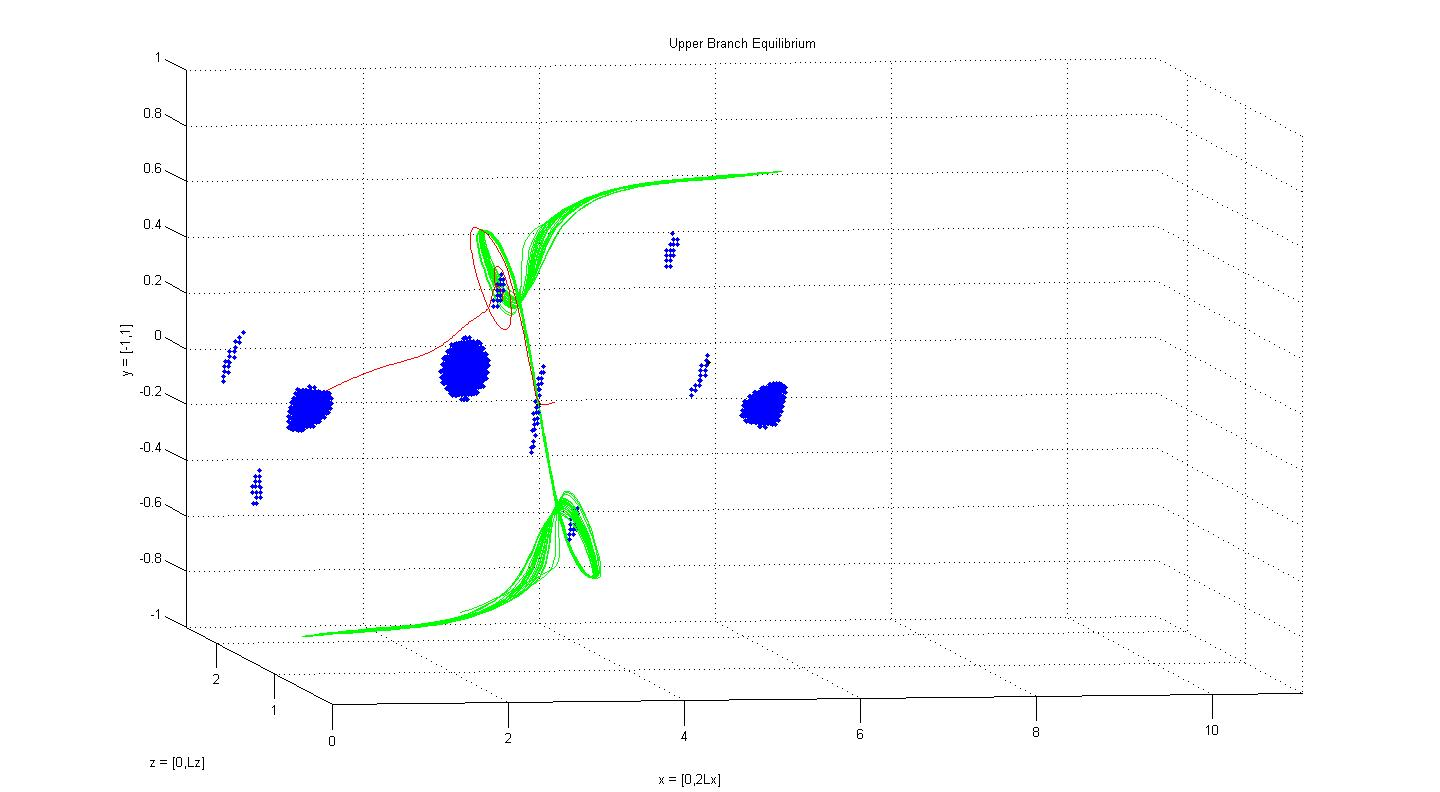
\includegraphics[width=0.95\textwidth]{fine_usquare.jpg}
  \caption{
Blue clumps of points indicate where the velocity for {\tEQtwo} is very 
close to zero. Shown along with the stable manifold of \tSP{3} and the 
unstable manifold of \tSP{1}. 
          }
  \label{fig:fine_usquare}
 \end{figure}
\end{center}

Repeating the linear stability analysis for \tSP{N1} and \tSP{N2}: 
There is one real, positive eigenvalue and a complex pair with negative 
real part. 
  \bea \eigExp[1] &=& 0.1453207 \,,\quad \jEigvec[1] =
\left[\begin{array}{c}
             {0.9307982} \cr
             {0.3502306} \cr
             {0.1046576} \cr
\end{array}\right]
   \continue
\{ \eigExp[2],\eigExp[3]\}
  &=& \eigRe[2] \pm i \,\eigIm[2] =  -0.0726603 \pm i\, 0.3733478
   \continue
\jEigvec[2]  &=&
\left[\begin{array}{c}
             {~0.5226203} \cr
             {-0.6703938} \cr
             {~0.2065610} \cr
\end{array}\right]
    \,,\quad
\jEigvec[3] =
\left[\begin{array}{c}
             {~0.3779843} \cr
             {~
             0} \cr
             {- 0.3031510} \cr
\end{array}\right]
\,.
\nnu
\eea
The \velgradmat\ is
\[ %beq
   {\Mvar} =
\left[\begin{array}{ccc}
   {0.0225166} &  {0.0985763} &{0.7623083} \cr
   {0.1714566} &   {-0.1275193} & {-0.6118476} \cr
   {-0.0615378}  &   {0.1755954}  & {0.1050028} \cr
         \end{array}\right]
\,.
\] %eeq

We have this time a $1D$ unstable manifold and a $2D$ spiraling stable 
manifold. The trajectories shown in \reffig{fig:fine_usquare}, which 
originate close to \tSP{1} and \tSP{3}, wander close to the spiraling stable 
manifold of the numerically discovered \tSP{N1}, showing how the 
dynamics tends to be dominated by these {\stagp}s. 

 \begin{figure}
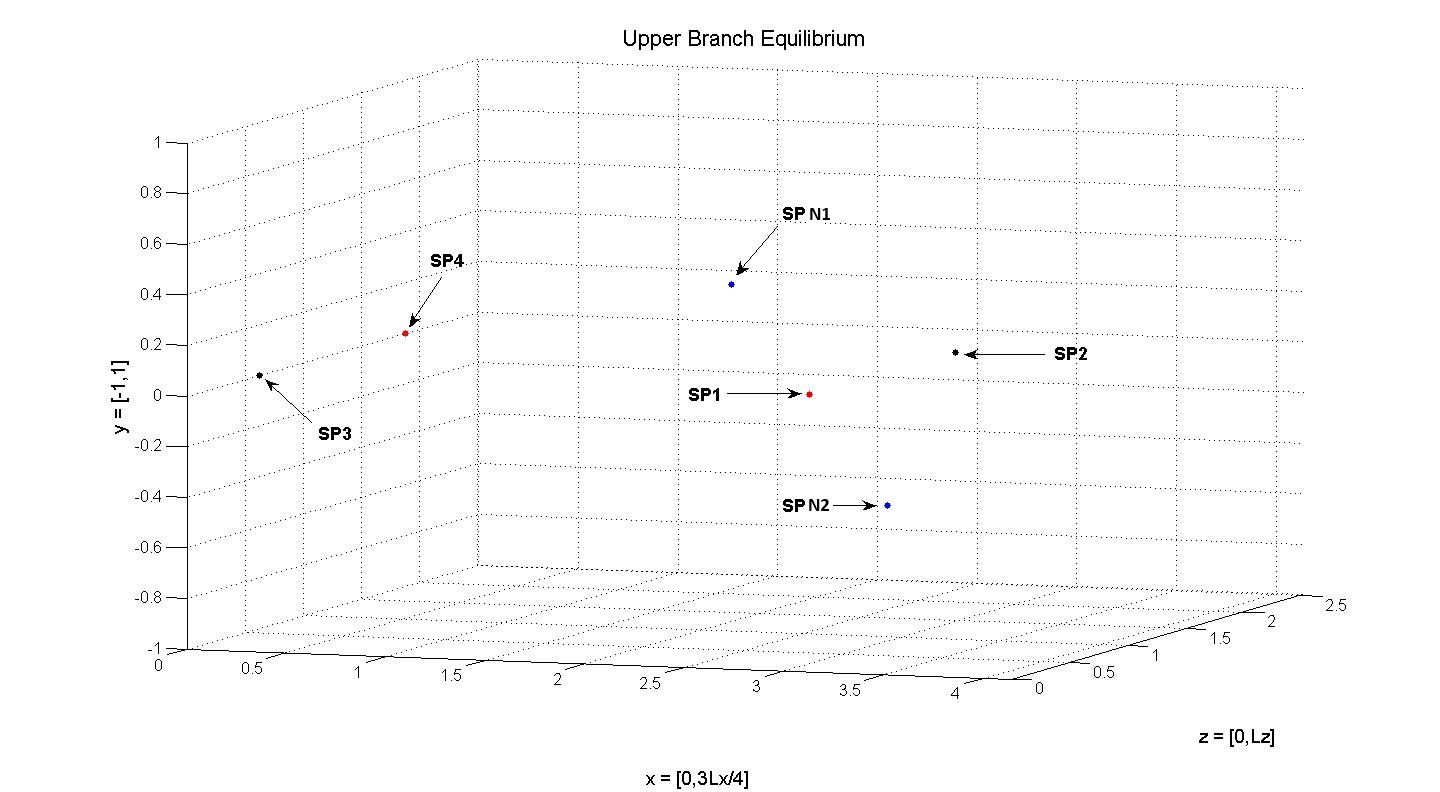
\includegraphics[width=0.95\textwidth]{stagps_edited.jpg}
  \caption{
   The 6 unique \stagp s within one periodic box for {\tEQtwo}. 
   \tSP{1}--\tSP{4} are guaranteed by {\tEQtwo} symmetries, \tSP{N1} and 
   \tSP{N2} are determined numerically. 
   }
  \label{fig:stagps_label}
 \end{figure}

 \begin{figure}
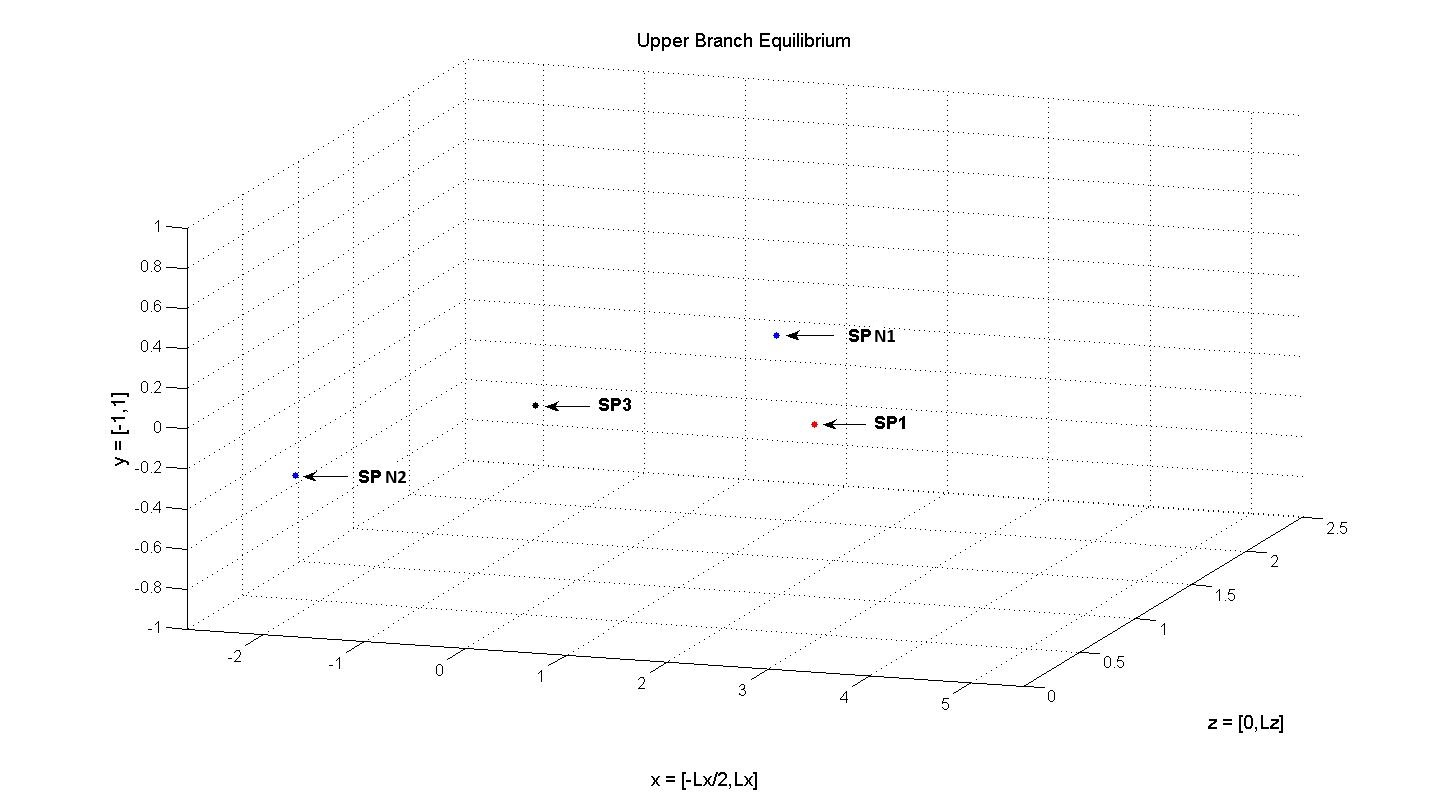
\includegraphics[width=0.95\textwidth]{stagps2_edited.jpg}
  \caption{
   The 4 \stagp s that occur within the domain $\Omega$.
   }
  \label{fig:stagps_label2}
 \end{figure}

We have been describing all \stagp s which are inside a single periodic 
cell with dimensions $L_x \times 2 \times L_z$, pictured in 
\reffig{fig:stagps_label}. However even within this cell there is a 
redundancy in labeling all of these points as distinct. The interesting 
dynamics and connections between the different \stagp s occur along the 
$x$ direction. To understand what is happening one needs to look only at 
a subset of these \stagp s that lies in the right or left half of the 
box, that is, in the interval $[0,L_{z}/2]$ or the interval 
$[L_{z}/2,L_{z}]$. We have chosen the interval $[0,L_{z}/2]$. In the $x$ 
direction the most convenient interval is not actually $[0,L_{x}]$, 
rather we look at the \stagp s in the open interval $(-L_{x}/2,L_{x})$, 
open so as to ignore the repeated translations on the boundary. Thus an 
alternate domain of investigation that will be convenient to sometimes 
use is 
\[ %beq 
\Omega = (-L_{x}/2,L_{x}) \times [-1,1] \times [0,L_{z}/2]
\,. 
\] %eeq 
Within this domain $\Omega$ there are then just four \stagp s. They 
are \tSP{1}, \tSP{3}, \tSP{N1}, and \tSP{N2}, shown in 
\reffig{fig:stagps_label2}. Note that \tSP{N2} is a translated 
version from the way it was viewed in \reffig{fig:stagps_label}. The 
phase portrait of fundamental dynamics for {\tEQtwo} will be viewed in 
$\Omega$.


\subsection{A colorful flow portrait and {\hc}s}

With identification of all of the {\stagp}s within either the original 
periodic box or the cell $\Omega$, as well as the corresponding linear 
stability analysis, we are ready to make a complete phase space portrait 
for the upper branch, {\tEQtwo}.

\begin{figure}
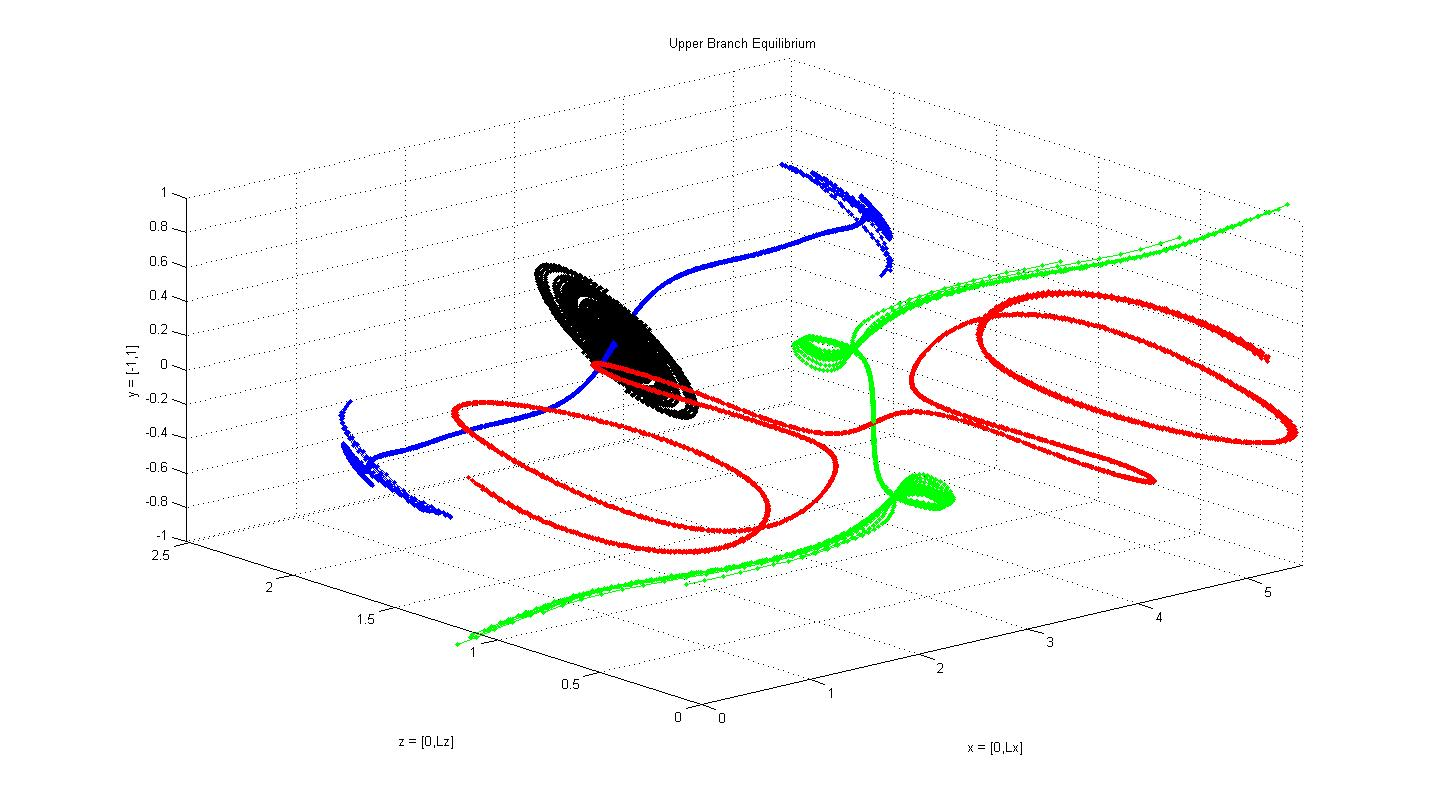
\includegraphics[width=0.95\textwidth]{manifolds_both.jpg}
  \caption{
   Segments of the stable (red/blue) and unstable (green/black) manifolds of the \stagp s
   $\xSP{1} = (L_x/2,0,L_z/4)$ and
   $\xSP{2} = (L_x/2,0,3L_z/4)$ for {\tEQtwo}. 
   }
  \label{fig:manifolds_both}
 \end{figure}


    \begin{figure}
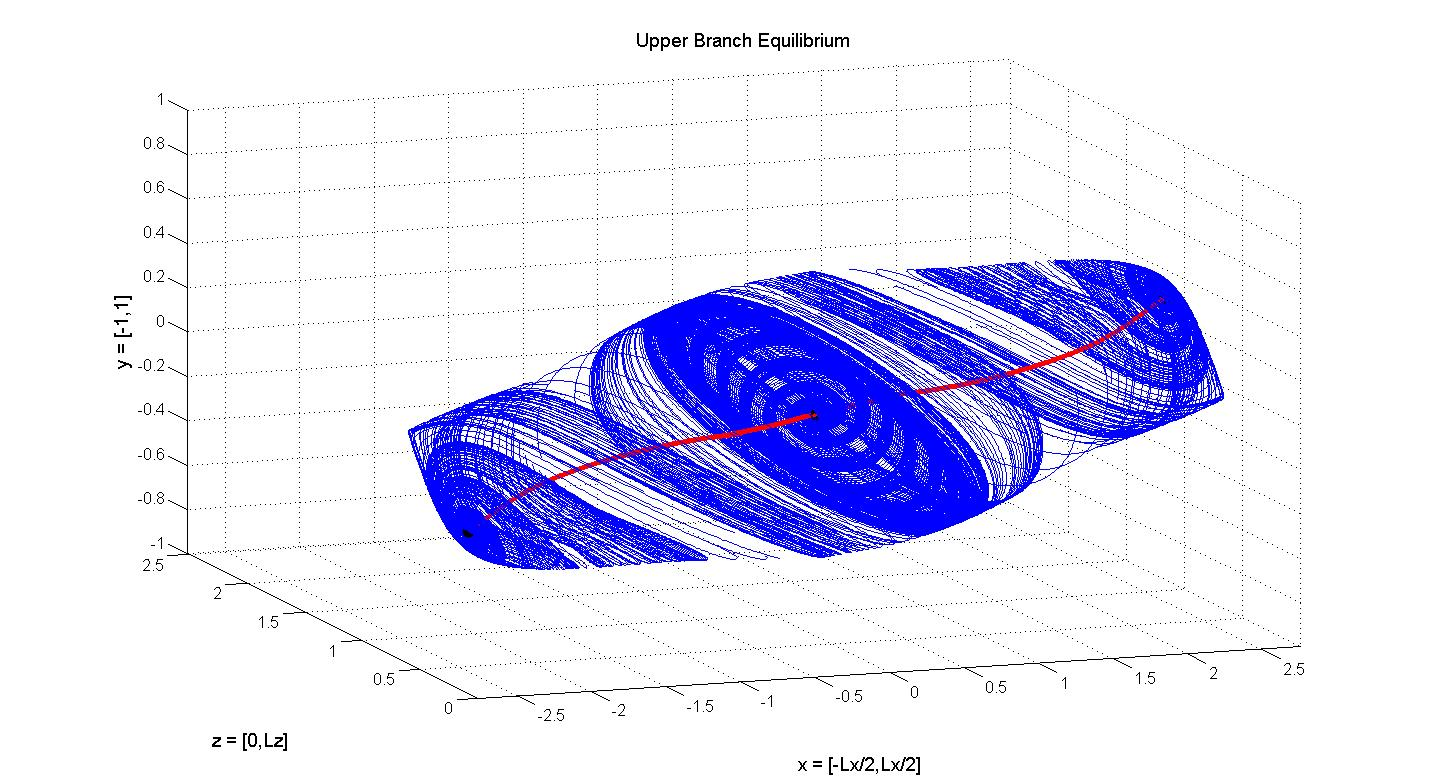
\includegraphics[width=0.95\textwidth]{man14_june3.jpg}
  \caption{
{\Hec}s of the upper branch (red trajectories) from 
$\tSP{N1} \to \tSP{3}$ and $\tSP{N2} \to \tSP{3}$, shown in a cell with $x \in$ 
[-$L_x/2$, $L_x/2$] along with the unstable manifold of \tSP{3}. 
   }
  \label{fig:hetero1}
 \end{figure}

  \begin{figure}
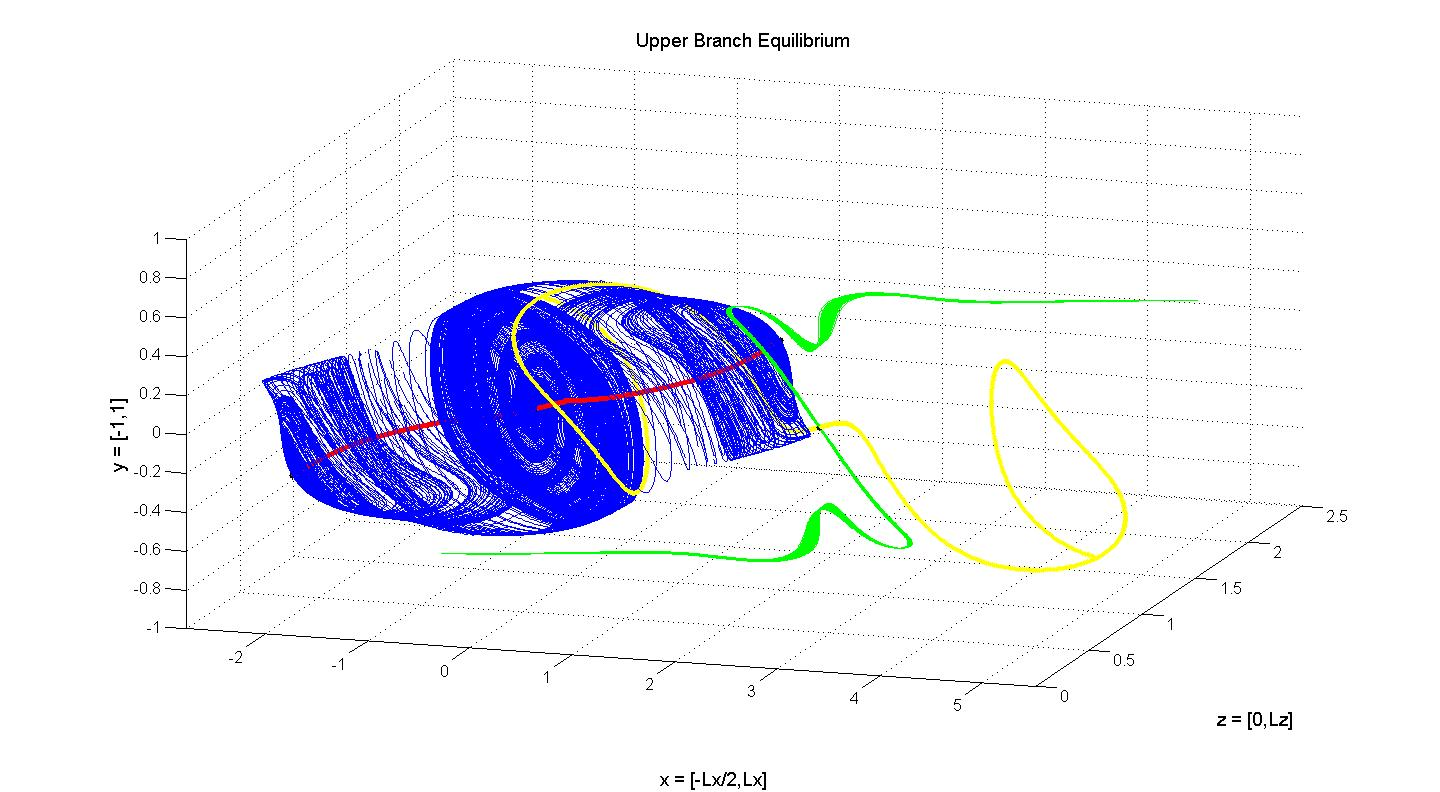
\includegraphics[width=0.95\textwidth]{june4_fig7.jpg}
  \caption{
Portrait of the fundamental dynamics along the manifolds of \stagp s 
\tSP{1}, \tSP{3}, \tSP{N1}, \tSP{N2} within cell $\Omega$ for the upper 
branch. 
   }
  \label{fig:hetero2}
 \end{figure}

The dynamics between the \stagp s and their translations is quite 
interesting. In \reffig{fig:manifolds_both} we see a partial view of 
the stable and unstable manifolds of two of the {\stagp}s, \tSP{1} and 
\tSP{2}, in the original periodic domain, found by integrating 
trajectories near the fixed points forwards and backwards in time along 
the stable or unstable eigenvectors. Local stability analysis shows that 
\tSP{1} has all real eigenvalues with a $1D$ stable manifold, and a $2D$ 
unstable manifold which is locally a plane 
\refeq{sp1_evec1}-\refeq{sp1_evec3}. The fact that one of the eigenvalues 
for the unstable manifold of \tSP{1} is much larger than the other is 
apparent in the figure by the fact that the trajectories in the unstable 
plane become quickly contracted in one of the dimensions, and the 
trajectories appear to leave along a nearly one-dimensional structure in 
the $y$-direction. \tSP{2} has a $2D$ unstable manifold with complex 
eigenvalues which spiral out in a plane and a $1D$ stable manifold. 
 
As alluded to in \reffig{fig:fine_usquare}, \tSP{N1} and \tSP{N2} 
sit near the center of the swirl of green coming from the unstable 
direction of \tSP{1}. To better understand what is happening here, 
referring to \reffig{fig:hetero1}, we compute the  stable and 
unstable manifolds of \tSP{N1} and \tSP{N2}, where we use the shifted 
translation of \tSP{N2}, along with the stable and unstable manifolds of 
\tSP{3}. The blue surface is formed by the overlap of trajectories 
starting along the unstable manifold of \tSP{3} and the stable manifolds 
of \tSP{N1} and \tSP{N2}.  We see that the stable manifold of \tSP{3} 
(shown by the red curves) corresponds with the unstable manifolds of 
\tSP{N1} and \tSP{N2}, thus we have \emph{{\hc}s} from $\tSP{N1}\to\tSP{3}$
 and $\tSP{N2}\to\tSP{3}$! The thick appearance of the red curves 
is simply so that they can be seen within the blue surface. They are 
actually just a single trajectory. 
 
Next we bring trajectories originating near \tSP{1} into the picture to 
see how the manifolds of this {\stagp} connect with those in 
\reffig{fig:hetero1}, producing the full dynamical portrait within 
$\Omega$.  The result is shown in \reffig{fig:hetero2}. Compare to 
\reffig{fig:stagps_label2} to see the locations of the {\stagp}s. 
The relation of the stable manifold of \tSP{1} (yellow curve) and the 
trajectories that are driven away from \tSP{1} in the unstable direction 
(green) to those of the blue surface is significant. These 
trajectories tightly hug the blue surface as they spiral around it, 
appearing to be shielded from entering the volume it encompasses. This 
has important implications for the consideration of fluid mixing 
within {\pCf},  showing that it is difficult to achieve a 
uniformly mixed space for this particular Eulerian equilibrium; a blob of ink that 
starts outside of the blue surface will have a difficult time ever 
entering the region! 
 
One merely translates the image in \reffig{fig:hetero2} in the $x$ 
direction by an amount $L_{x}$ to give a complete picture in any periodic 
cell. The same picture will also occur symmetrically (translated by 
$L_{x}/2$ and $L_{z}/2$) in the left half of the box. 


\subsection{Eulerian equilibrium {\tEQeight}: additional symmetries}
\label{sect:EQ8}

Having analyzed the upper branch Eulerian equilibrium {\tEQtwo}, we next look at 
{\tEQeight}, another Eulerian equilibrium velocity field of {\pCf} which exhibits 
turbulent behavior at a lower Reynolds number, 270.


We start once again with a cleverly chosen grid of initial trajectories 
to get a feel for the significant structures in the flow. The grid is in 
a plane at $x = L_{x}/2$. The result, after a short integration time, is 
shown in \reffig{fig:EQ8_grid1}. This perspective view already shows 
us quite a bit of information. Once again we have symmetries abound, and 
we know from the discussion in \refsect{s:symm_stag} that there will be 
at least 8 {\stagp}s \tSP{1}--\tSP{8}.  Another interesting feature of this 
plot is the four vortical structures on the left half. One final 
noteworthy point from the figure is the appearance of a perfect line 
segment connecting two of the {\stagp}s, which happen to be \tSP{1} and 
\tSP{2}. This strongly suggests a heteroclinic connection between these 
two \stagp s. To confirm, we compute the eigenvalues and eigenvectors of 
the \velgradmat. For \tSP{1}, there is indeed a real, unstable eigenvector 
pointing along (0,0,1) and for \tSP{2} there is a real, stable eigenvector 
pointing along (0,0,1). This, together with the plot, numerically 
confirms the existence of the heteroclinic trajectory. The same result  
holds for the shifted pair at $x = 0$. The rest of the 
eigenvalues/eigenvectors are given below. We note that for {\tEQeight} there 
is a {\hc} which is a simple horizontal line connecting the pair of 
trivial \stagp s in the \emph{spanwise} direction, whereas for \tEQtwo\ 
the connection was some arbitrary-looking curve in the 
\emph{streamwise} direction connected to a nontrivial \stagp. 
Factorization of the \tSP{1} and \tSP{2} stability eigenspaces for {\tEQeight} 
occurs because the spanwise $z$ direction is a $1D$ flow-invariant 
subspace at the \stagp s \citep{SiCvi10}. That ensures the simplicity of 
the \hec. 

{\tEQeight}, \tSP{1}: There are two real, positive eigenvalues
 and one real, negative eigenvalue.
\bea
\left(
    \eigExp[1],\eigExp[2],\eigExp[3]
\right) &=&
      (0.363557,0.227831,-0.591389)
\label{E8SP1} \\
\left(
    \jEigvec[1],\jEigvec[2],\jEigvec[3]
\right) &=&
\left(
    \left[\begin{array}{c}
             {0} \cr
             {0} \cr
             {1}
 \end{array}\right] \,,
    \left[\begin{array}{c}
             {-0.733415} \cr
             {-0.679780} \cr
             {0}
 \end{array}\right] \,,
    \left[\begin{array}{c}
             {0.991005} \cr
             {0.133824} \cr
             {0}
 \end{array}\right]
\right) \,.
\nnu
\eea

{\tEQeight}, \tSP{2}: There are two real, positive eigenvalues
 and one real, negative eigenvalue.
\bea
\left(
    \eigExp[1],\eigExp[2],\eigExp[3]
\right) &=&
      (0.992857,0.255973,-1.248830)
\label{E8SP2} \\
\left(
    \jEigvec[1],\jEigvec[2],\jEigvec[3]
\right) &=&
\left(
    \left[\begin{array}{c}
             {~0.116961} \cr
             {-0.993136} \cr
             {0}
 \end{array}\right] \,,
    \left[\begin{array}{c}
             {0.957795} \cr
             {0.287450} \cr
             {0}
 \end{array}\right] \,,
    \left[\begin{array}{c}
             {0} \cr
             {0} \cr
             {1}
 \end{array}\right]
\right) \,.
\nnu
\eea


   \begin{figure}
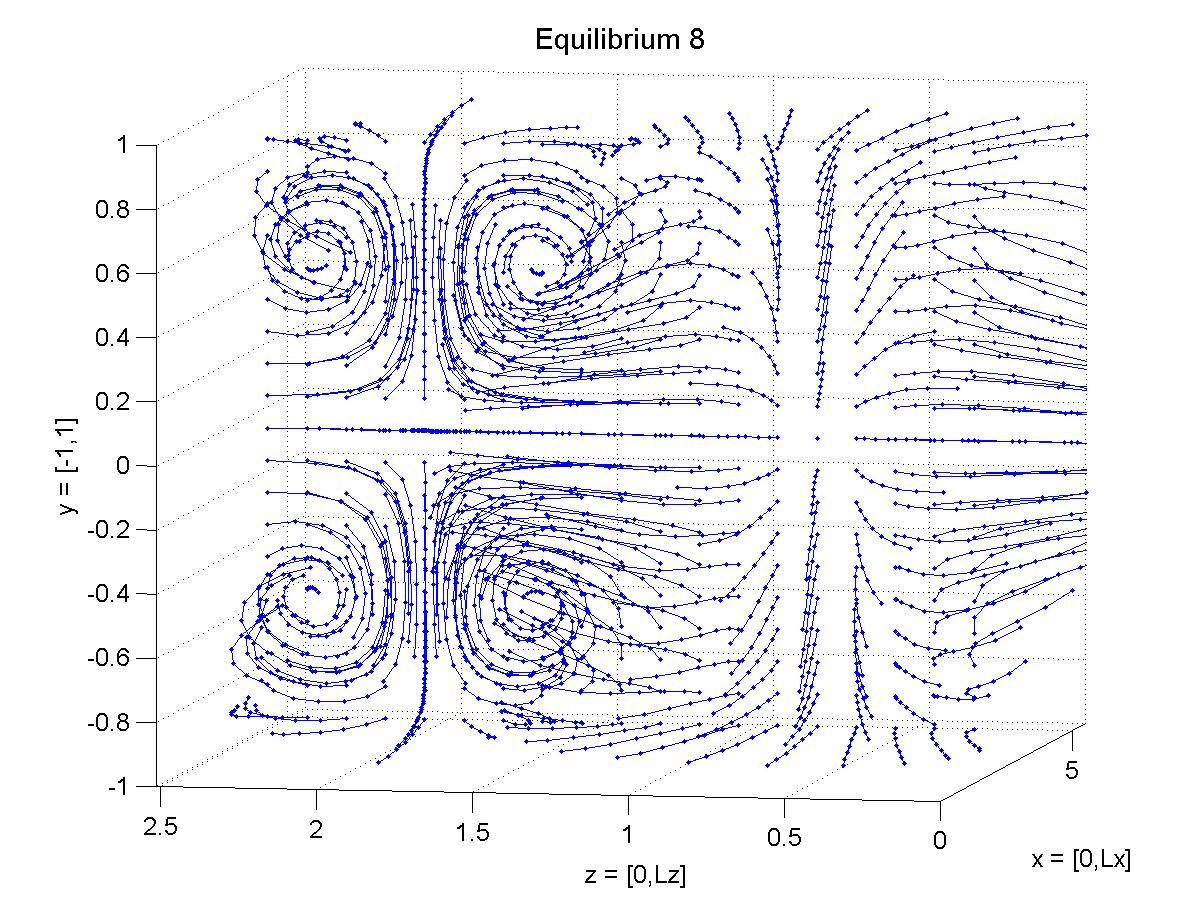
\includegraphics[width=0.9\textwidth]{EQ8_grid1.jpg}
  \caption{
    Grid of initial points in the $[y,z]$ plane, centered at $x = L_x/2$; 
    integrated to produce tracer particle trajectories for {\tEQeight}. 
   }
  \label{fig:EQ8_grid1}
 \end{figure}


Equilibrium {\tEQeight} (as well as {\tEQsev}, not discussed here), possesses 
additional symmetries compared to {\tEQtwo}. {\tEQtwo} is in the $S$-invariant 
subspace of velocity fields and {\tEQeight} is in $S_8$ (\refsect{s:PCF_symm}
and \refsect{s:symm_stag}). 

From \refeq{second_condition} and \refeq{s3lagrange} we know then that 
for {\tEQeight} we will have the additional {\stagp}s: 
 \bea
  \xSP{5} &=& (L_x/4,0,0) \continue
  \xSP{6} &=& (3L_x/4,0,0) \continue
  \xSP{7} &=& (L_x/4,0,L_z/2)  \\
  \xSP{8} &=& (3L_x/4,0,L_z/2) \nnu
 \,.
\eea
Interestingly these were actually discovered numerically \emph{before} 
the symmetry arguments were understood. A Newton search on regions of 
very low velocity for {\tEQeight} revealed that $(L_x/4,0,L_z/2)$ and 
$(3L_x/4,0,L_z/2)$ are \stagp s. From this, one may deduce that symmetry 
$s_5$ must hold, and it can then be checked that at any position the 
velocity field is indeed invariant under $s_4$ and $s_5$. 

Stability analysis of the additional set of {\stagp}s for {\tEQeight} gives the
following.

 \tSP{5}: There is one real, positive eigenvalue
 and a complex pair with negative real part.
\bea 
  \eigExp[1] &=& 0.03109 \,,\quad \jEigvec[1] =
\left[\begin{array}{c}
             {0.85275} \cr
             {0.41774} \cr
             {-0.31355} \cr
\end{array}\right]
   \continue
\{ \eigExp[2],\eigExp[3]\}
   &=& \eigRe[2] \pm i \,\eigIm[2] =  -0.01555 \pm i\, 0.59385
   \label{EQSP5eigs}\\
\jEigvec[2]  &=& 
\left[\begin{array}{c}
             {~0.24762} \cr
             {-0.31442} \cr
             {~0.69906} \cr
\end{array}\right]
    \,,\quad
\jEigvec[3] =
\left[\begin{array}{c}
             {-0.20793} \cr
             {~0.55489} \cr
             {~0} \cr
\end{array}\right]
\,.
\nnu
\eea
 We have a $1D$ unstable manifold and a $2D$ inward-spiral
stable manifold. All four of the new points have the same
eigenvalues. \tSP{5} and \tSP{8} have the same eigenvectors, as do \tSP{6}
and \tSP{7} whose eigenvectors differ from \tSP{5} only by the sign of
the third component for \jEigvec[1] and by the sign of the first and
second components for \jEigvec[2] and \jEigvec[3].

As a final interesting consequence of numerically searching for \stagp s 
for {\tEQeight}, the figures produced by plotting gridpoints where velocity is 
small, using a cutoff value of $|\mathbf{u}|^{2}$ which is too large to 
actually be useful for finding \stagp s, we instead find a plot showing 
more intricate patterns in the flow. \reffig{fig:usquare_EQ8_1} 
shows a $3D$ perspective view of these points, and 
\reffig{fig:usquare_EQ8_2} shows the projection of 
\reffig{fig:usquare_EQ8_1} onto the $xz$ plane. This 
volume-preserving flow (area preserving in Poincar\'e sections) may have 
invariant tori which, being quasiperiodic, would not be detected by the 
{\stagp} searching routines. Though the structures in the 
projection plot in \reffig{fig:usquare_EQ8_2} are not actual tracer 
trajectories, they are suggestive that a search for such invariant tori 
in future work may be a fruitful endeavor.  

\begin{figure}
\centering
    \begin{subfigure}{0.9\textwidth}
    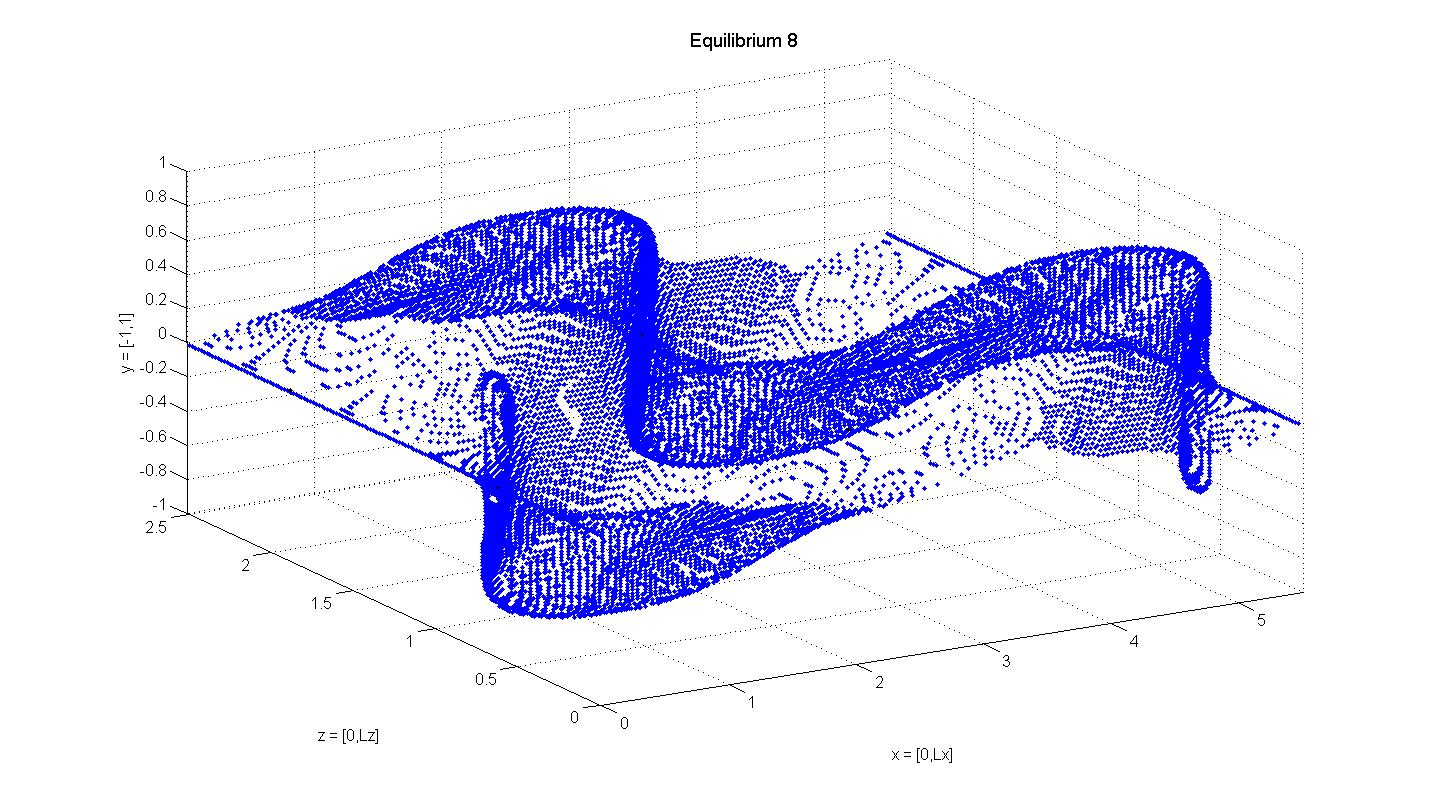
\includegraphics[width=1.0\textwidth]{usquare_EQ8_cute1.jpg}
      \caption{
        Perspective view.
       }
      \label{fig:usquare_EQ8_1}
    \end{subfigure}

    \begin{subfigure}{0.9\textwidth}
    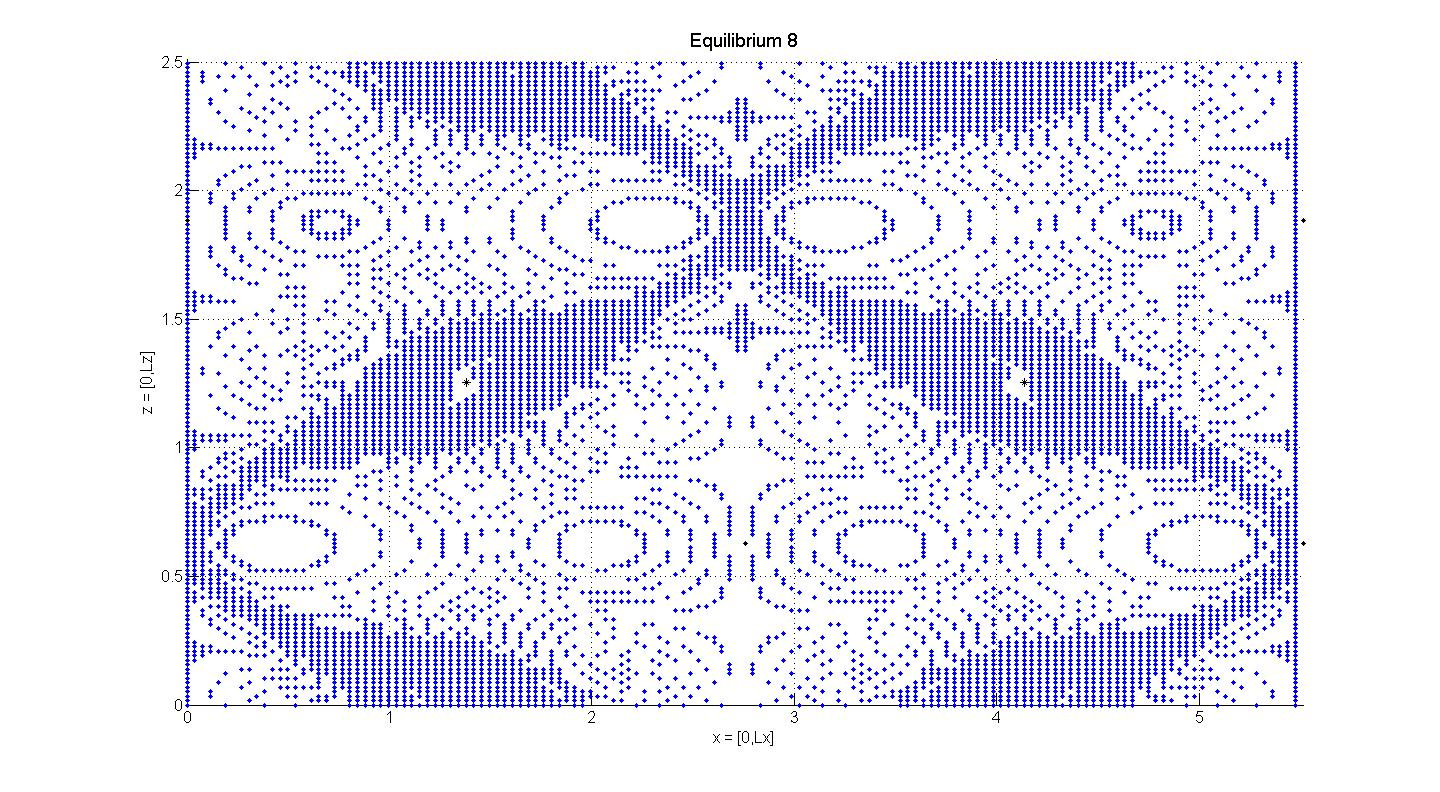
\includegraphics[width=1.0\textwidth]{usquare_EQ8_cute2.jpg}
      \caption{
       Projection onto the $xz$
       plane.
       }
      \label{fig:usquare_EQ8_2}
    \end{subfigure}  
    \caption{
A plot of points where the velocity field falls below a small cutoff for 
{\tEQeight}, showing interesting structures in the flow. 
       }
    \label{fig:usquare_both}
 \end{figure}

